\documentclass[12pt]{article}
\usepackage{amsmath}
\usepackage{graphicx}
\usepackage{caption}
\usepackage{subcaption}
\usepackage{booktabs}
\usepackage{float}
\usepackage[utf8]{inputenc}
\usepackage{geometry}
\usepackage{multirow}
\usepackage{setspace}
\usepackage{parskip}
\usepackage{svg}
\usepackage[bottom]{footmisc}
\usepackage{tikz}
\usepackage[section]{placeins}
\usepackage{minted}
% This style is used to create block diagrams, you'll find it useful since many of your figures would be of that form, I'll try add more styles in the future :)
\usetikzlibrary{trees,positioning,fit,calc}
\tikzset{block/.style = {draw, fill=blue!20, rectangle,
                         minimum height=3em, minimum width=4em},
        input/.style = {coordinate},
        output/.style = {coordinate}
}

\usepackage{minted}
\usepackage{chngcntr}
\counterwithin{figure}{section}

\renewcommand{\arraystretch}{1.5}

\usepackage[hidelinks]{hyperref}
\hypersetup{
    linktoc=all
}

\renewcommand\listingscaption{Listing}
\renewcommand\listoflistingscaption{List of Listings}

\usepackage{scrhack}
\usepackage{tocbasic}
\setuptoc{lol}{levelup}

\usepackage{indentfirst}
\geometry{a4paper, margin=1in}

%----------EDIT COVER INFO HERE -----------------%
\def \LOGOPATH {assets/ru}
\def \UNIVERSITY { University of Rajshahi}
\def \DEPARTEMENT {Department of Computer Science \&  Engineering}
\def \COURSENUM {CSE4182}
\def \COURSENAME {Digital Image Processing Lab}
\def \REPORTTITLE {Explaining Fourier Transformation effect on image}
\def \STUDENTNAME {Abdur Rahim Sheikh}
\def \STUDENTID {1810576141}
\def \INSTRUCTOR {Sangeeta Biswas, associate professor}

%------------------------------------------------%

\setlength{\parindent}{0em}
\setlength{\parskip}{0em}

\begin{document}

\pagenumbering{Roman}

\begin{titlepage}
    \vfill
    \begin{center}
        \includesvg[width=0.4\textwidth]{\LOGOPATH} \\
        \hfill \\
        \Huge {\UNIVERSITY} \\
        \Large{\DEPARTEMENT} \\
        \Large{\COURSENUM\;-\;\COURSENAME} \\
        \vfill
        \textbf{\LARGE{\REPORTTITLE}}
    \end{center}
    \vfill
    \begin{center}
        \Large{\textbf{Prepared by:} \STUDENTNAME} \\
        \textbf{student id:} \STUDENTID \\
        \Large{\textbf{Instructor:} \INSTRUCTOR} \\
        \Large{\textbf{Date:} \today}
    \end{center}
    \vfill
\end{titlepage}

%--------------ABSTRACT ------------------------%
{
\centering
\section*{Abstract}
The Fourier Transform is used to work if signal as well as image in frequency domain. And a fastest version of Fourier Transform which is fft (Fast Fourier Transform) can be used to work with any signal in frequency domain with minimal time complexity and more flexibility.
}
%-----------------------------------------------%
\clearpage
\tableofcontents
\clearpage

\setlength{\parskip}{\baselineskip}%

\pagenumbering{arabic}

%--------------INTRODUCTION ---------------------%

\section{Introduction}

To understand the effect of Fourier Transform we need an image and here is the image I chose to apply fast Fourier transform.
\begin{figure}[H]
    \centering
    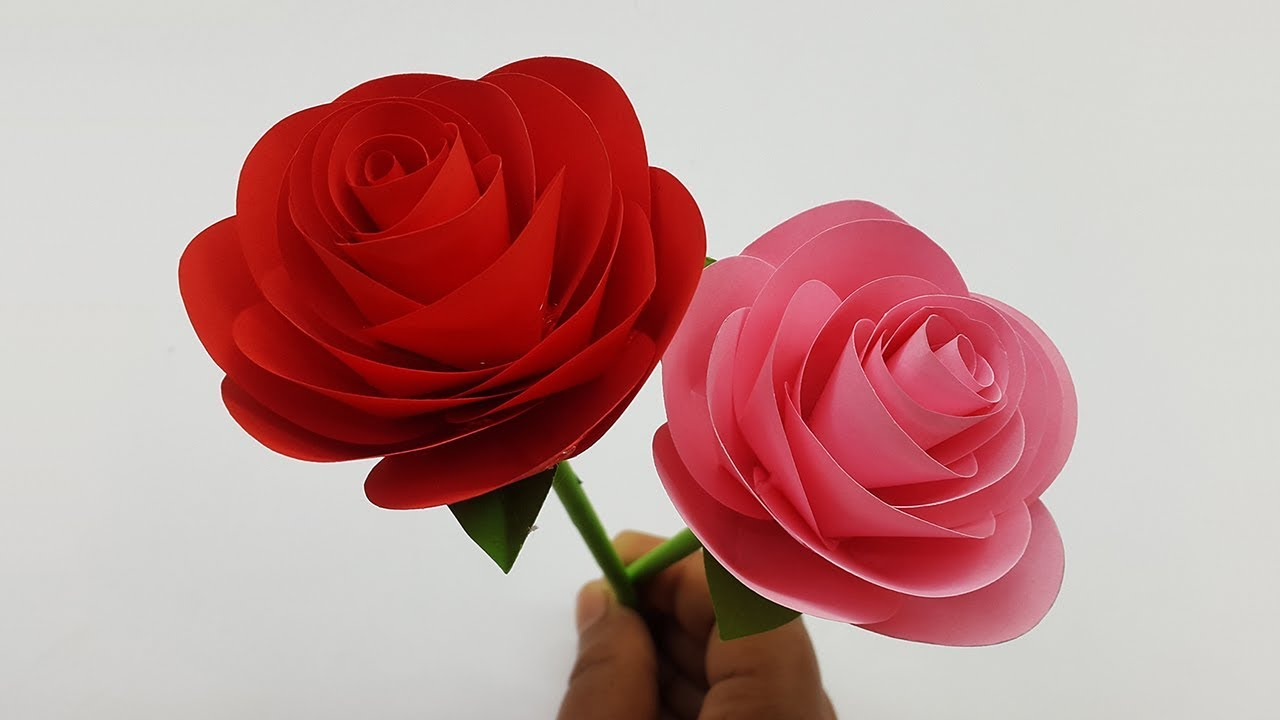
\includegraphics[width=.6\textwidth]{assets/rose.jpg}
    \caption{red rose}
    \label{fig:smile}
\end{figure}

\section{Methods}
This is an RGB image. We will apply Fourier Transform in a gray-scale image. To convert gray-scale we will use the python module OpenCV called cv2.
\subsection{Transform to Gray-scale}

\begin{minted}{python}
img = plt.imread('rose.jpg')
src_img = cv2.cvtColor(img,cv2.COLOR_RGB2GRAY)
plt.imshow(src_img)
\end{minted}

\subsection{Fourier Transform}
In this report, we used Numpy's built-in function FFT2 (2 because our image is a 2D signal). Then centered the Fourier transformed image by using "fftshift" function. Then, we will calculate the magnitude spectrum.

\begin{minted}{python}
fftImg = np.fft.fft2(src_img)
centerImg = np.fft.fftshift(fftImg)
centerImgLog = 100 * np.log(abs(centerImg))
\end{minted}

\subsection{Filters}
I created 4 filter kind of arbitary but those are 3 rectengle of different size and one circle.

\clearpage

\subsubsection{Filter1}
It's a 100 by 100 rectangle in the center.

\begin{minted}{python}
filter1 = np.zeros((r,c),np.uint8)
filter1= cv2.rectangle(filter1,(oy-50,ox-50),(oy+50,ox+50),(255,255,255),-1)
imageBack1 = centerImg * filter1
filterImg1 = np.abs(np.fft.ifft2(imageBack1))
\end{minted}
Output:

\begin{figure}[H]
    \centering
    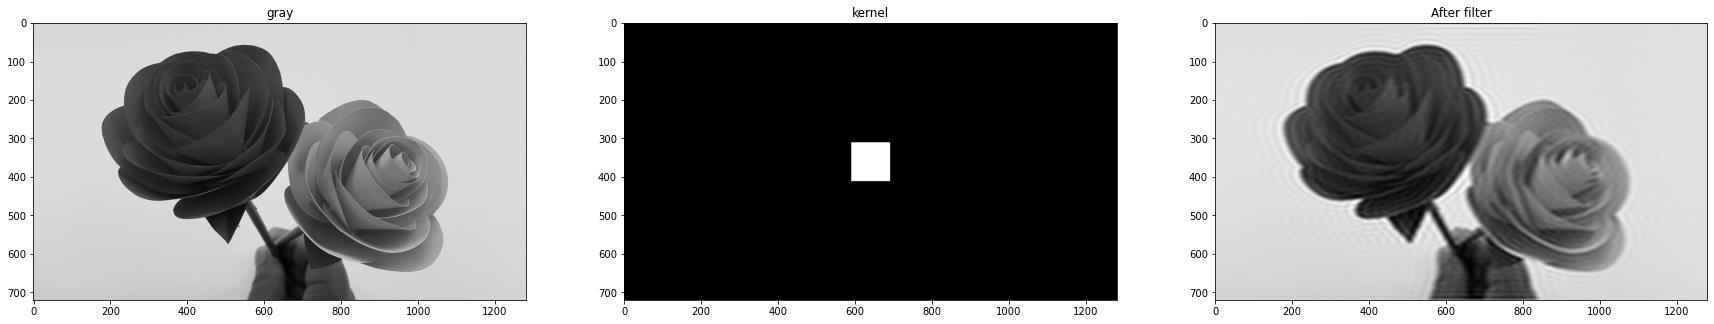
\includegraphics[width=1\textwidth]{assets/kernel1_transform.jpg}
    \caption{Filter 1 applied in frequency domain(Fourier Transformed)}
    \label{fig:Filter1}
\end{figure}


Analysis: there is some circular glow around the image.
\clearpage


\subsubsection{Filter2}
This filter is a circle in the center.

\begin{minted}{python}
filter2 = np.zeros((r,c),np.uint8)
filter2 = cv2.circle(filter2,(oy,ox),70,(255,255,255),-1)
imageBack2 = centerImg * filter2
filterImg2 = np.abs(np.fft.ifft2(imageBack2))
\end{minted}

Output:

\begin{figure}[H]
    \centering
    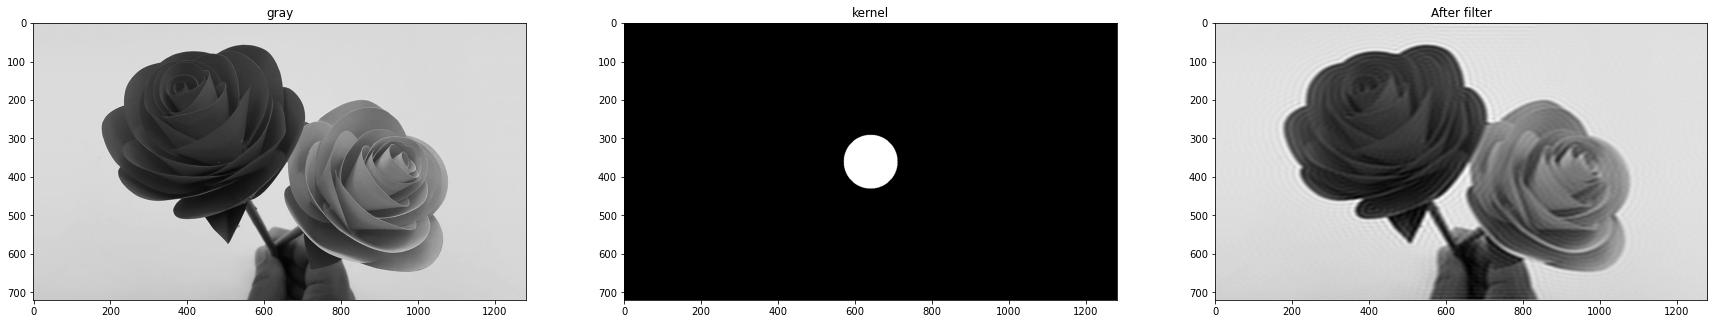
\includegraphics[width=1\textwidth]{assets/kernel2_transform.jpg}
    \caption{Filter 2 applied in frequency domain(Fourier Transformed)}
    \label{fig:Filter2}
\end{figure}


Analysis: This also have circular glow but it's more sharp then the rectangle.

\clearpage




\subsubsection{Filter3}
The idea was to create a filter that contained half of all the values 1 and the others zero (axis=column). It is the same as above but the difference is we applied it with a column axis.

\begin{minted}{python}
filter3 = np.zeros((r,c),np.uint8)
filter3[:oy,:] = 1
imageBack3 = centerImg * filter3
filterImg3 = np.abs(np.fft.ifft2(imageBack3))
\end{minted}
Output:

\begin{figure}[H]
    \centering
    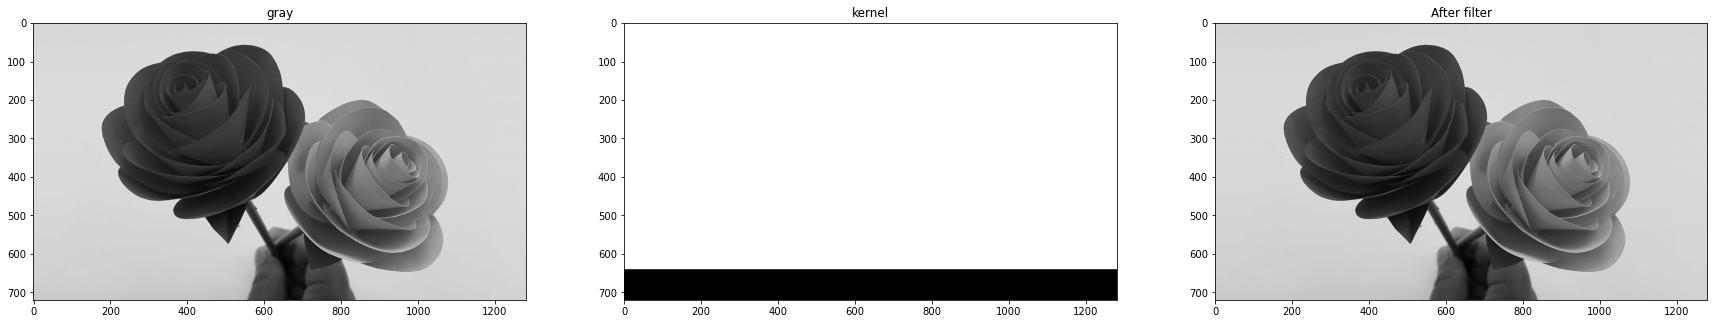
\includegraphics[width=1\textwidth]{assets/kernel3_transform.jpg}
    \caption{Filter 3 applied in frequency domain(Fourier Transformed)}
    \label{fig:Filter3}
\end{figure}


Analysis: No effect seen.

\clearpage

\subsubsection{Filter4}
It's another rectangle.

\begin{minted}{python}
filter4 = np.zeros((r,c),np.uint8)
filter4[:ox+30,:oy+90] = 1
imageBack4 = centerImg * filter4
filterImg4 = np.abs(np.fft.ifft2(imageBack4))
\end{minted}

Output:

\begin{figure}[H]
    \centering
    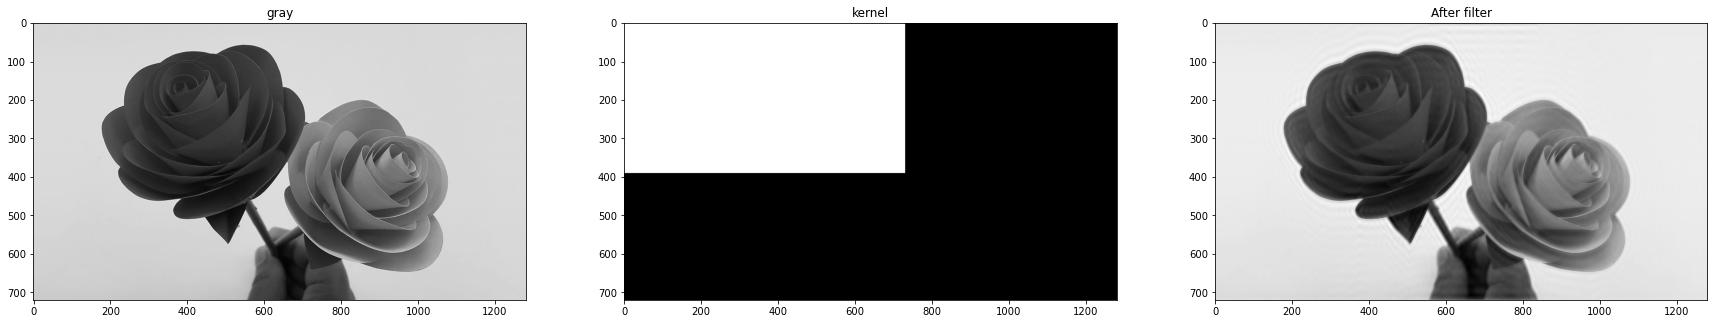
\includegraphics[width=1\textwidth]{assets/kernel4_transform.jpg}
    \caption{Filter 4 applied in the frequency domain(Fourier Transformed)}
    \label{fig:Filter5}
\end{figure}

\clearpage
\section{Conclusion}
The main advantage of Fourier transform is that we can apply filters in the frequency domain. And it's time complexity is less. So it's a great tool to filter images and do other application with it.

\clearpage

\section{visualization code}
\begin{minted}{python}
def show_transformation(gray,kernel,filtered,img_name):
plt.figure(figsize=(30,20))
def plot_it(img,title,ind):
    plt.subplot(1,3,ind)
    plt.imshow(img,cmap='gray')
    plt.title(title)
    
plot_it(gray,'gray',1)
plot_it(kernel,'kernel',2)
plot_it(filtered,'After filter',3)
plt.savefig(img_name,bbox_inches='tight')
plt.show()
\end{minted}

\listoffigures

\end{document}